% !TEX root =  ../main_manuscript.tex

\section{Results}
\label{sec:results}
From the joint model fitted to the PRIAS dataset, we found that both $\log_2 \{\mbox{PSA} + 1\}$ velocity,  and log odds of having $\mbox{DRE} > \mbox{T1c}$  were significantly associated with the hazard of cancer progression. For any patient, an increase in $\log_2 \{\mbox{PSA} + 1\}$ velocity from -0.03 to 0.16 (first and third quartiles of the fitted velocities, respectively) corresponds to a 1.94 fold increase in the hazard of cancer progression. Whereas, an increase in odds of $\mbox{DRE} > \mbox{T1c}$ from 0.001 to 0.01 (first and third quartiles of the fitted odds, respectively) corresponds to a 1.40 fold increase in the hazard of cancer progression. Detailed results pertaining to the fitted joint model are presented in Appendix B.

\subsection{Comparison of Various Approaches for Biopsies}
From the simulation study, we obtain the number of biopsies and the delay in detection of cancer progression for each of the ${\mbox{500} \times \mbox{250}}$ test patients using different schedules. Figure \ref{fig:better_balance_results} shows that the personalized and PRIAS approaches fall in the region of better balance between the number of biopsies and the delay, than fixed/heuristic schedules. We next evaluate these schedules on the basis of both median and interquartile range (IQR) of the number of biopsies and delay (see Figure~\ref{fig:sim_res_combined}). For brevity, only the most widely used annual and PRIAS schedules, the proposed personalized approach with fixed risk thresholds of 5\% and 10\%, and visit-specific threshold chosen using $\mbox{F}_1$ score are discussed next (see Appendix~C for remaining).

\begin{figure}[!htb]
\captionsetup{justification=justified}
\centerline{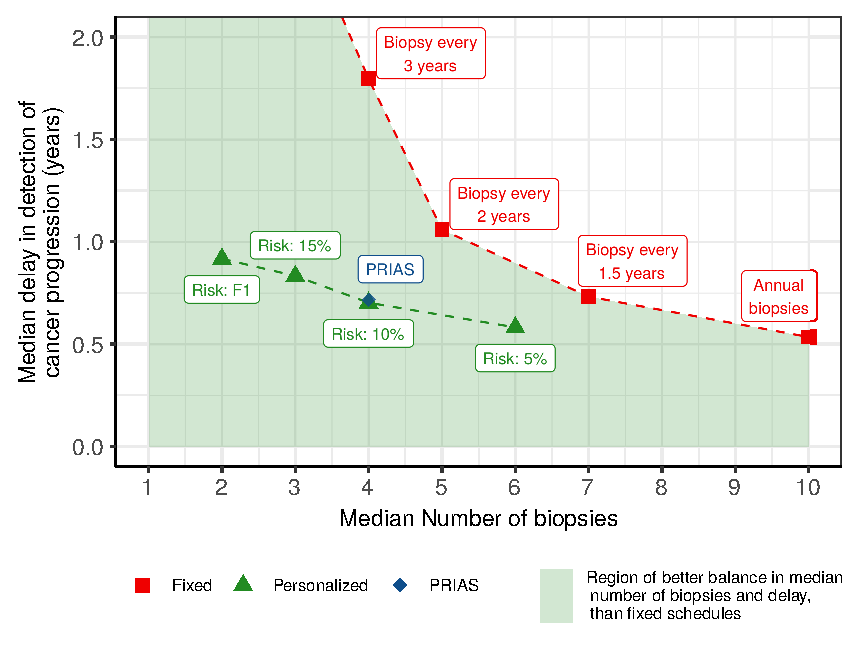
\includegraphics[width=\columnwidth]{images/better_balance_results.eps}}
\caption{\textbf{Simulation study results for burden-biopsy frontier:} Estimated median number of biopsies, and median delay in detection of cancer progression, due to the currently practiced fixed/heuristic biopsy schedules (red squares) and PRIAS schedule (blue rhombus), and personalized schedules (green triangles), over a follow-up of ten years. \textbf{Types of personalized schedules:} Risk:~15\%, Risk:~10\% and Risk:~5\% approaches, schedule biopsy if the cumulative risk of cancer progression at a visit is more than 15\%, 10\% and 5\%, respectively. Risk:~F1 works similar as previous, except that a visit-specific risk threshold is chosen by maximizing $\mbox{F}_1$ score (see \hyperref[sec:methods]{Methods}). The green shaded region depicts the region of better balance in number of biopsies and delay, than the currently practiced fixed/heuristic schedules. Estimation is based on results obtained from the simulation study we conducted. }
\label{fig:better_balance_results}
\end{figure}

Since patients have varying cancer progression speeds, the impact of each schedule also varies with it. In order to highlight these differences, we divide results for three types of patients, as per their time of cancer progression. They are \textit{fast, intermediate,} and \textit{slow progressing} patients. Although such a division may be imperfect and can only be done retrospectively in a simulation setting, we do it only for the purpose of illustration. Roughly 50\% of the patients did not obtain cancer progression in the ten year follow-up period of the simulation study. We assume these patients to be \textit{slow progressing} patients. We assume \textit{fast progressing} patients are the ones with an initially misdiagnosed state of cancer \cite{cooperberg2011outcomes}, or high-risk patients who choose AS instead of immediate treatment upon diagnosis. These are roughly 30\% of the population, having a cancer progression time less than 3.5 years. We label the remaining 20\% patients as \textit{intermediate progressing} patients. 

\begin{figure}[!htb]
\captionsetup{justification=justified}
\centerline{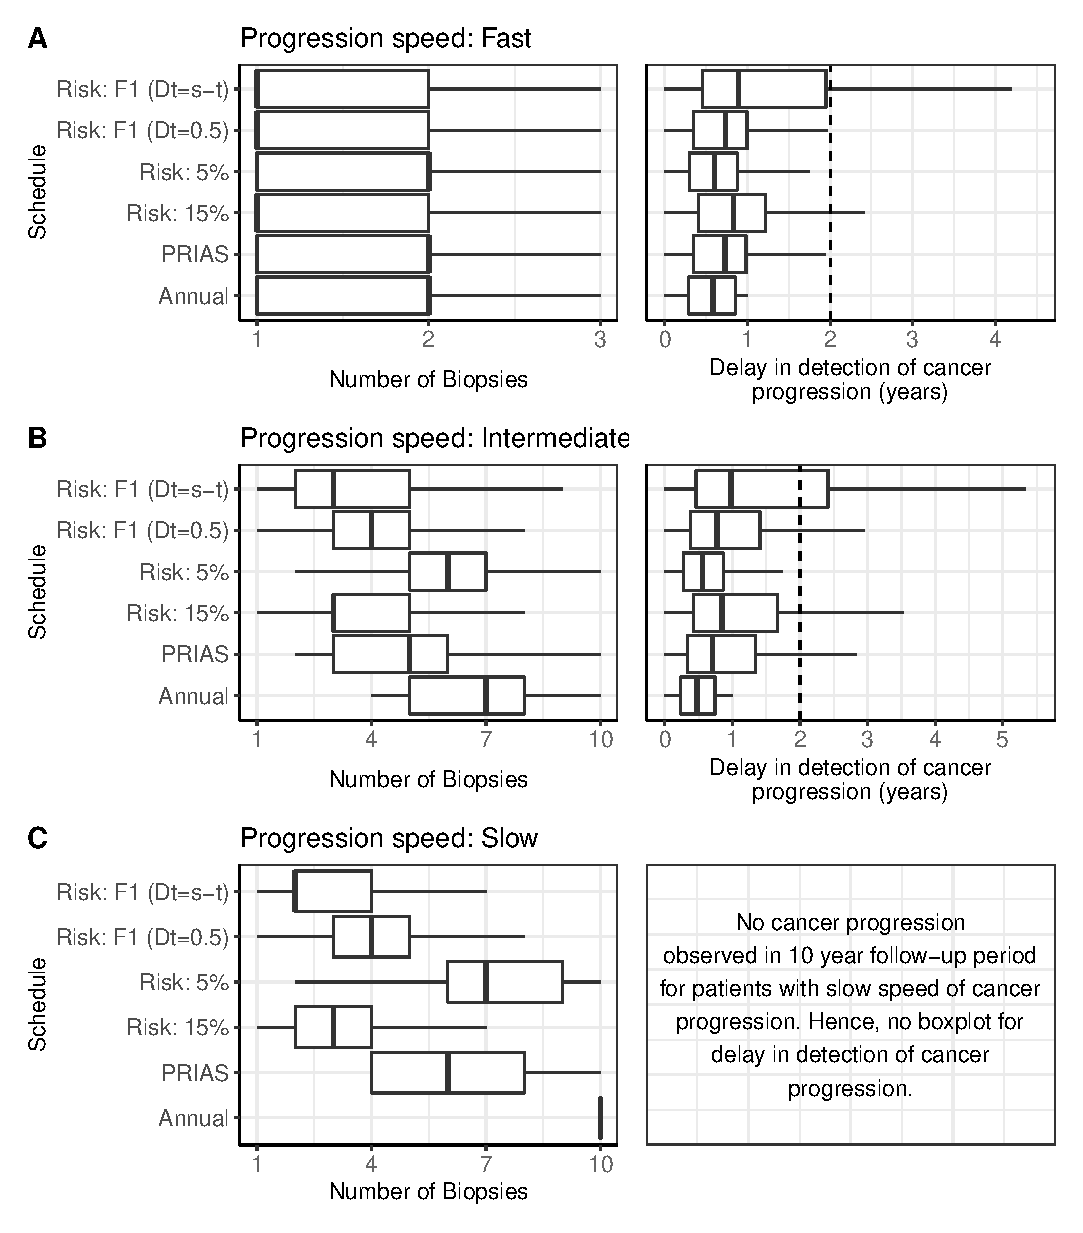
\includegraphics[width=\columnwidth]{images/sim_res_combined.eps}}
\caption{Boxplot showing variation in the number of biopsies, and the delay in detection of cancer progression, in years (time of positive biopsy - true time of cancer progression) for various biopsy schedules. Biopsies are conducted until cancer progression is detected. \textbf{Panel~A:} results for simulated patients who had a faster speed of cancer progression, with progression times between 0 and 3.5 years. \textbf{Panel~B:} results for simulated patients who had an intermediate speed of cancer progression, with progression times between 3.5 and 10 years. \textbf{Panel~C:} results for simulated patients who did not have cancer progression in the ten years of follow-up. \textbf{Types of personalized schedules:} Risk:~10\% and Risk:~5\% approaches, schedule biopsy if the cumulative risk of cancer progression at a visit is more than 10\% and 5\%, respectively. Risk:~F1 works similar as previous, except that a visit-specific risk threshold is chosen by maximizing $\mbox{F}_1$ score (see \hyperref[sec:methods]{Methods}). Annual corresponds to a schedule of yearly biopsies and PRIAS corresponds to biopsies as per PRIAS protocol (see \hyperref[sec:introduction]{Introduction}).}
\label{fig:sim_res_combined}
\end{figure}

 For \textit{fast progressing} patients (Panel~A,~Figure~\ref{fig:sim_res_combined}), we note that the personalized schedules with a fixed 10\% risk threshold and visit-specific threshold chosen using $\mbox{F}_1$ score, reduce one biopsy for 50\% of the patients, compared to PRIAS and annual schedule. Despite this, the delay is similar for personalized schedule with fixed 10\% risk threshold (median:~0.7~years,~IQR:~0.7~years), and the currently practiced annual (median:~0.6~years,~IQR:~0.6~years) and PRIAS schedules (median:~0.7~years,~IQR:~0.7~years).

For \textit{intermediate progressing} patients (Panel~A,~Figure~\ref{fig:sim_res_combined}), we note that the delay due to personalized schedule with fixed 5\% risk threshold (median:~0.6~years,~IQR:~0.6~years) is comparable to that of annual schedule (median 0.5~years,~IQR:~0.5~years). However, it schedules fewer biopsies (median:~6,~IQR:~2) than the annual schedule (median:~7,~IQR:~3). The delay for PRIAS (median:~0.7~years,~IQR:~1 year) and personalized schedule with fixed 10\% risk (median:~0.7,~IQR:~0.9) is similar, but the personalized approach schedules one less biopsy for 50\% of the patients. Although the approach with visit-specific risk threshold chosen using $\mbox{F}_1$ score schedules fewer biopsies than the 10\% fixed risk approach, but it also has a higher delay.

The patients who are at the most advantage with the personalized schedules are the \textit{slow progressing} patients. These are a total of 50\% patients who did not progress during the entire study. Hence, the delay is not available for these patients (Panel~C of Figure~\ref{fig:sim_res_combined}). For all of these patients, annual schedule leads to 10 (unnecessary) biopsies. The PRIAS schedule, schedules a median of 6 biopsies (IQR: 4). In comparison, the biopsies scheduled by the personalized schedules using fixed 10\% risk threshold (median:~4,~IQR:~2) and visit-specific risk chosen using $\mbox{F}_1$ score (median:~2,~IQR:~2), are much fewer.

Overall, we observed that the personalized schedule which uses 10\% risk threshold at all follow-up visits is dominant over the PRIAS schedule, biennial schedule of biopsies, and biopsies every one and a half years. This personalized schedule not only schedules less number of biopsies than the aforementioned currently practiced schedules, but the delay in detection of cancer progression is also either equal or less. The personalized schedule which uses risk threshold chosen on the basis of classification accuracy ($\mbox{F}_1$ score) is dominant over the triennial schedule of biopsies. The personalized schedule which uses 5\% risk threshold schedules less biopsies than the annual schedule, while the delay is only trivially more than the annual schedule.

